\part{Linear baseline model}
\label{part:linear_baseline}

%------------------------------------

\section{About this part}
\label{section:LBM_about_part}
A good linear model available in the SciKit Learn library is the Logistic Regression model.
This model is often used as a linear baseline model to compare other models with.
Only models scoring better then this linear baseline model should be considered.
This part discusses the parameters found to be optimal for this model in this setting and the road to finding these optimal parameters.
The Python-based Jupyter Notebook corresponding with this part is \texttt{linear\_baseline\_model.ipynb}.
This notebook will form a \emph{template} for future model exploration.
%------------------------------------

\section{Scoring used to evaluate the model}
\label{section:LBM_scoring_used}

The multi-class Log Loss score of a validation set taken from the training set is used to evaluate models.
This scoring strategy is the same as used in the Kaggle competition.
An important note to make is that the unbalance, as discussed in section \ref{section:DA_data_distribution}, might make this score overly dependent on classes which have many instances.
This can and will be taken into account for some settings.


%------------------------------------

\section{Fine-tuning the input}
\label{section:LBM_finetuning_clusters}
The first step in finding optimal settings for the model is finding optimal settings for the input of the model.
In this case, the parameters that can control the input are the number of clusters each image is separated into and the descriptor used as discussed in part \ref{part:data_analysis}.
In general, more clusters often correspond to a better score, however, including many clusters can lead to overfitting of the model.
The following values were tried to manually find an optimum:
\begin{itemize}
    \item Descriptors: DAISY, ORB, FREAK, LUCID, VGG, BoostDesc, SIFT.
    \item Cluster amounts (small): 5, 20, 50, 100, 150, 250 and 500.
    \item Cluster amounts (small): 500, 1000, 3000 and 5000.
\end{itemize}

A comparison was done by averaging the multi-class Log Loss score over 5 trials for each of these cluster amounts and descriptors.
Only the test score results are of significance.
There are 2 ways of looking at this data.
The descriptor that achieves the minimum with a certain cluster amount can be seen as the optimal setting.
However, since clustering is used, one can consider the \emph{elbow method} to determine the optimal setting as well.
Figure \ref{fig:2-input} shows the found results for all used descriptors and cluster amounts.
When taking into consideration the elbow method, the \emph{SIFT} descriptor performs best with a cluster amount around 100.
When looking at the minimum, it seems that the \emph{DAISY} descriptor would come out on top with a small margin.
The SIFT approach seems more viable since the difference in score is minimal and the SIFT approach uses less clusters suggesting it is more general.
In contrast, the Daisy approach has signs of overfitting.


\begin{figure*}[ht]
    \centering
    \begin{subfigure}{.45\textwidth}
        \centering
        \fbox{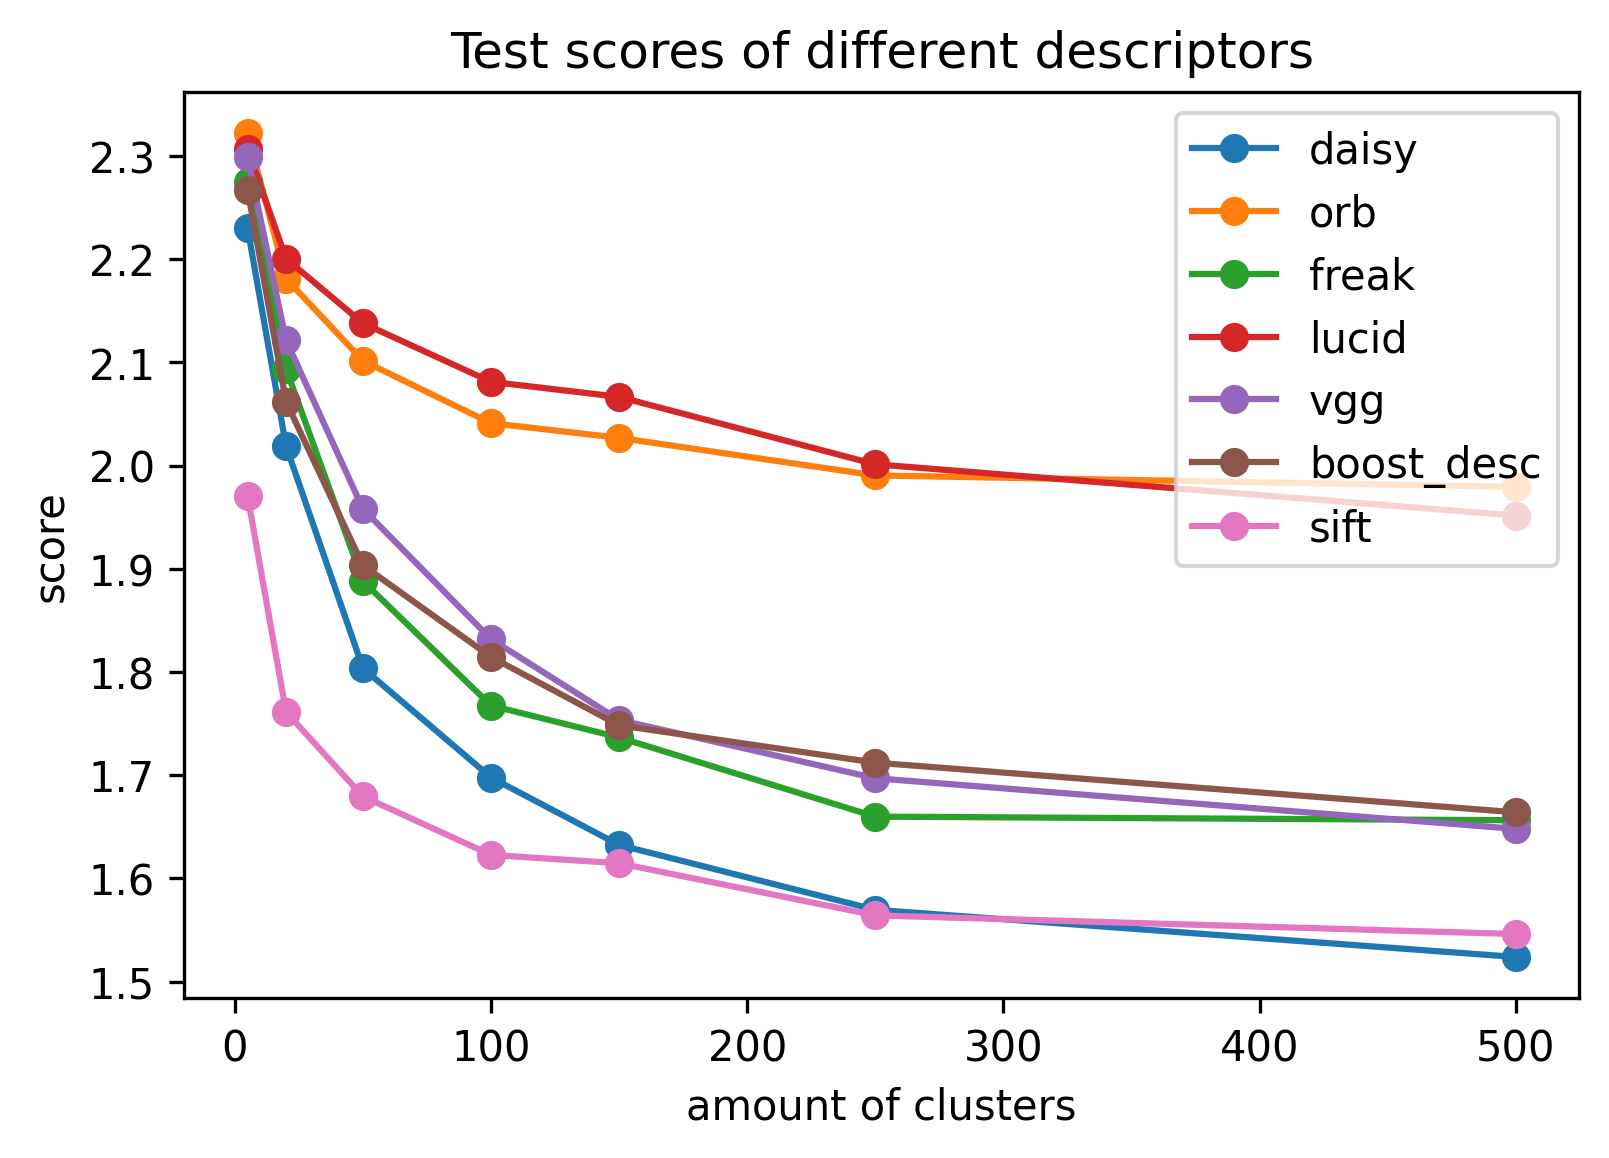
\includegraphics[width=\textwidth]{images/2/2-LBM-test_scores_all_small.png}}
        \captionsetup{width=0.9\linewidth}
        \captionsetup{justification=centering}
        \caption{Scores for small cluster amounts.}
    \end{subfigure}
    \hspace{1cm}
    \begin{subfigure}{.45\textwidth}
        \centering
        \fbox{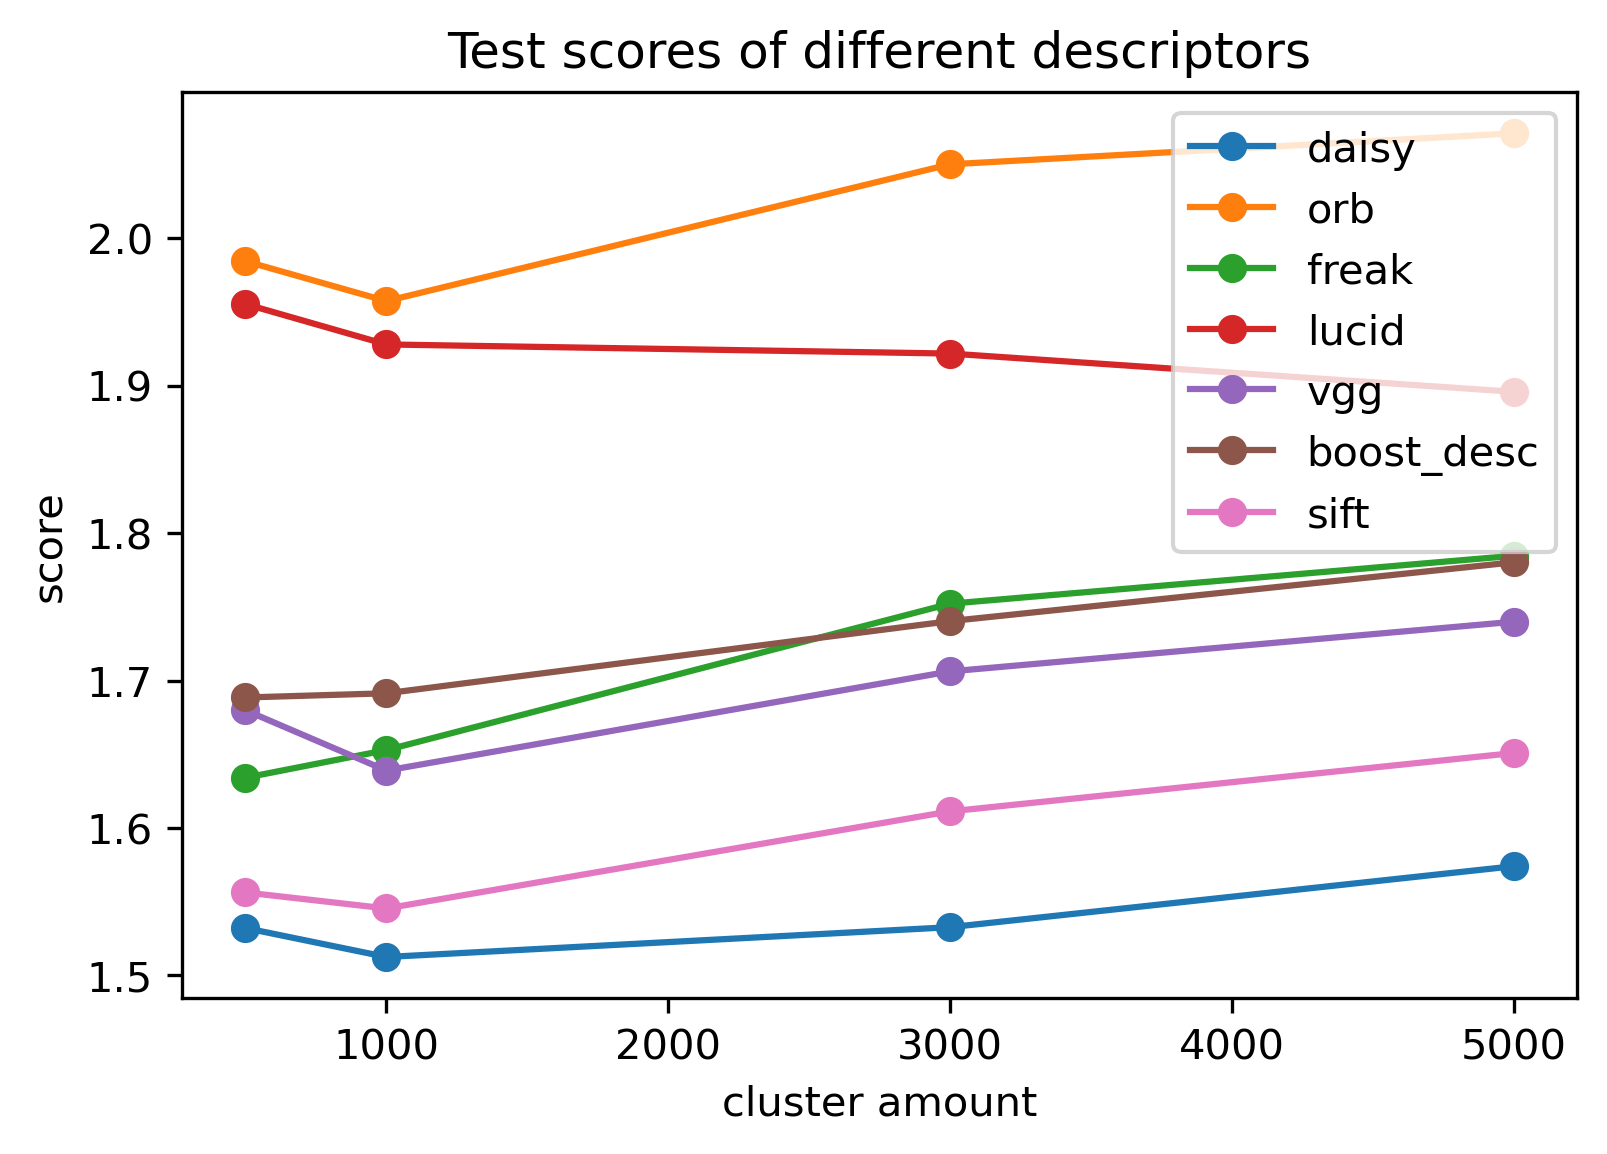
\includegraphics[width=\textwidth]{images/2/2-LBM-test_scores_all_large.png}}
        \captionsetup{width=0.9\linewidth}
        \captionsetup{justification=centering}
        \caption{Scores for large cluster amounts.}
    \end{subfigure}
    \captionsetup{width=0.8\linewidth}
    \captionsetup{justification=centering}
    \caption{Average multi-class Log Loss score over 5 trials for different descriptors and cluster amounts.}
    \label{fig:2-input}
\end{figure*}


%------------------------------------

\section{Fine-tuning the validation set}
\label{section:LBM_finetuning_validation_set}

\begin{wrapfigure}{r}{0.4\textwidth}
    \fbox{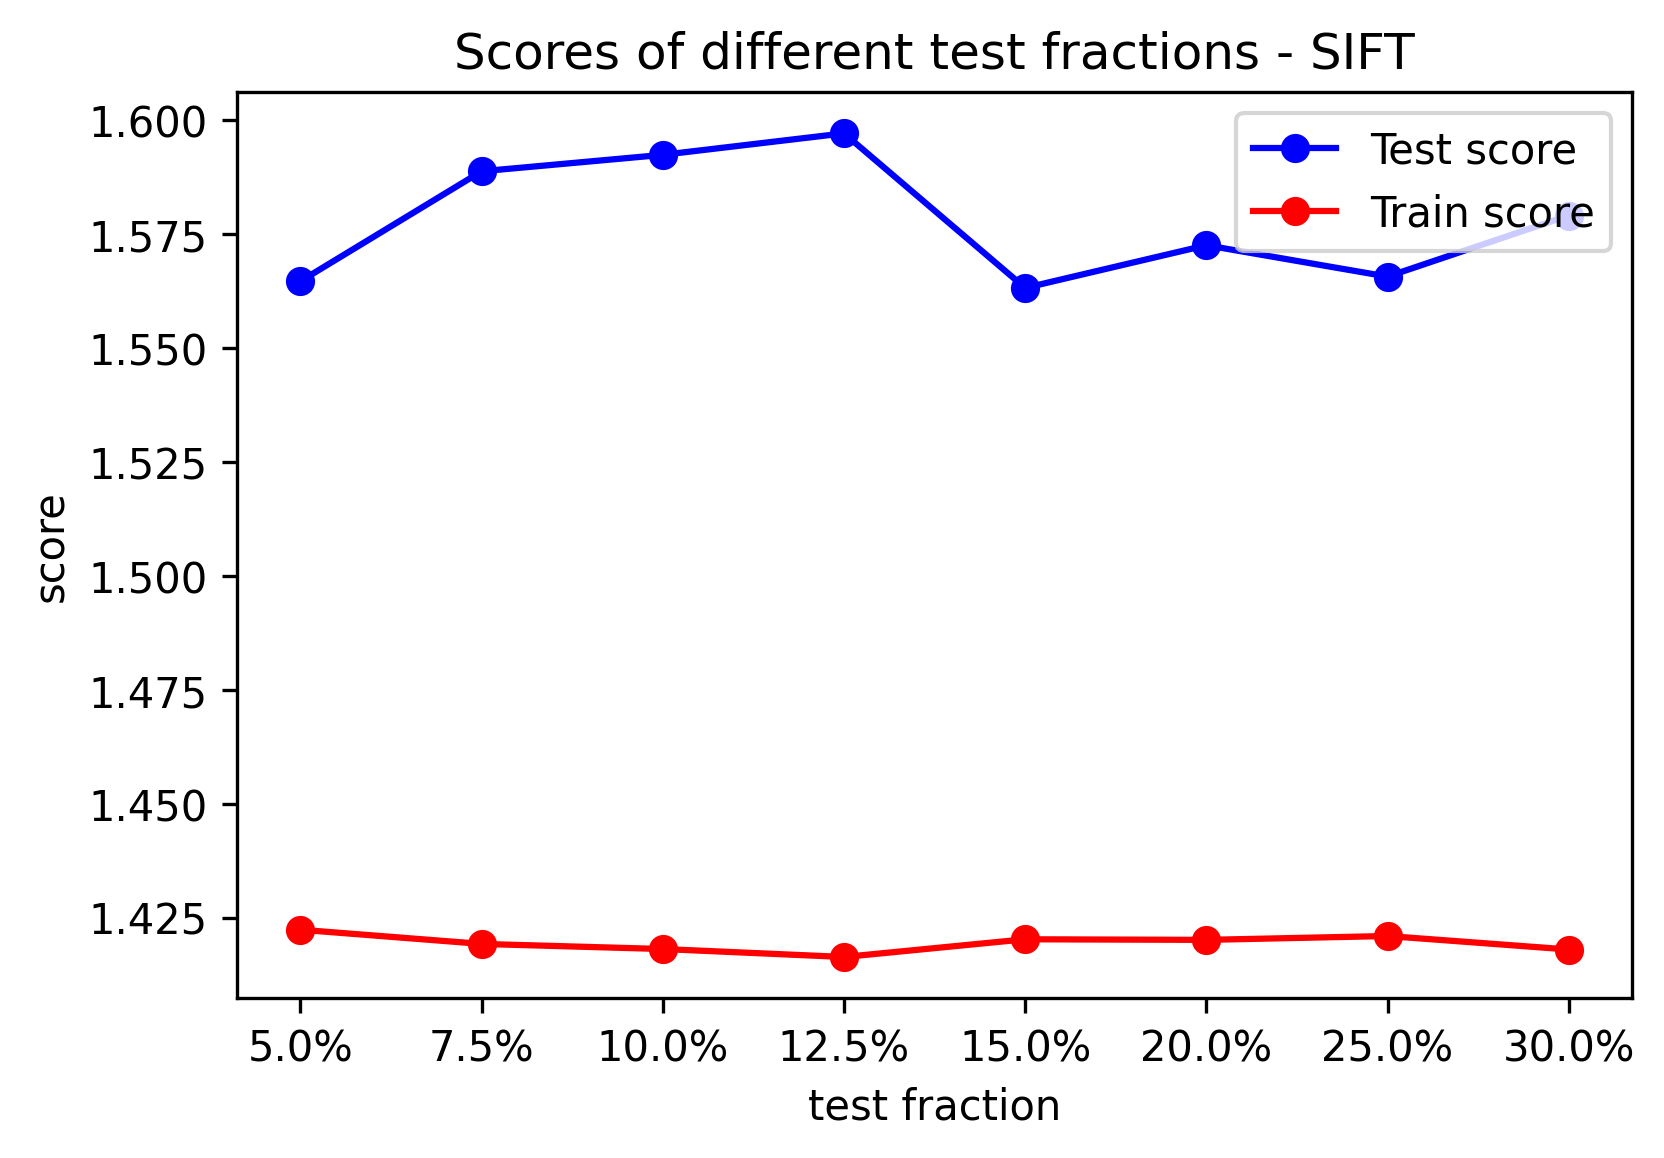
\includegraphics[width=0.9\linewidth]{images/2/2-LBM-test_size_sift.png}}
    \captionsetup{width=0.8\linewidth}
    \captionsetup{justification=centering}
    \caption{Experimenting with different test sizes.}
    \label{fig:2-LBM-test_size_sift}
\end{wrapfigure}

Since the training data is further split into a training and validation set, this splitting can also be fine-tuned.
The parameter that can be fine-tuned is \textit{test\_size} and whether or not to take into account that the data set is \textit{unbalanced}.
The latter is quite obvious as discussed in section \ref{section:DA_data_distribution} and thus the unbalance should be kept in mind.
Ideally, there would be enough instances in the training set to make a specific enough model and there would be enough models in the validation set to get a representative score. 
The following values test sizes were tested for the otherwise optimal settings: 5\%, 7.5\%, 10\%, 12.5\%, 15\%, 20\%, 25\%, 30\%.
Figure \ref{fig:2-LBM-test_size_sift} shows the result of this experiment using average multi-class Log Loss score over 5 trials.
A healthy balance seems to be around 15\%.



%------------------------------------

\section{Fine-tuning the model parameters}
\label{section:LBM_finetuning_model}

Now that all of the parameters available for the input are fine-tuned, the parameters of the model itself can be optimized.
As found in the documentation of the \texttt{LogisticRegression} function available in the SciKit Learn library there are multiple (optional) parameters \citep{scikit_learn}.
The most interesting ones are given in appendix B. 


Before experimenting, it was assumed that changing the class weight parameter to balanced would enhance the performance due to the unbalance of the training data.
Weirdly, this wasn't the case for the score received from the test set split from the training data nor on the Kaggle page.
Due to the unbalance the worse score for the split test set can be expected.
However, the fact that the score is worse on the Kaggle competition, 1.60289 vs 1.67565, is not expected.
Perhaps changing this parameter has more impact than was first assumed.
Setting the fit intercept parameter to false has a negative impact, albeit minor.
These experiments are visualised in figure \ref{fig:2-weightfit}.

\begin{figure*}[ht]
    \centering
    \begin{subfigure}{.45\textwidth}
        \centering
        \fbox{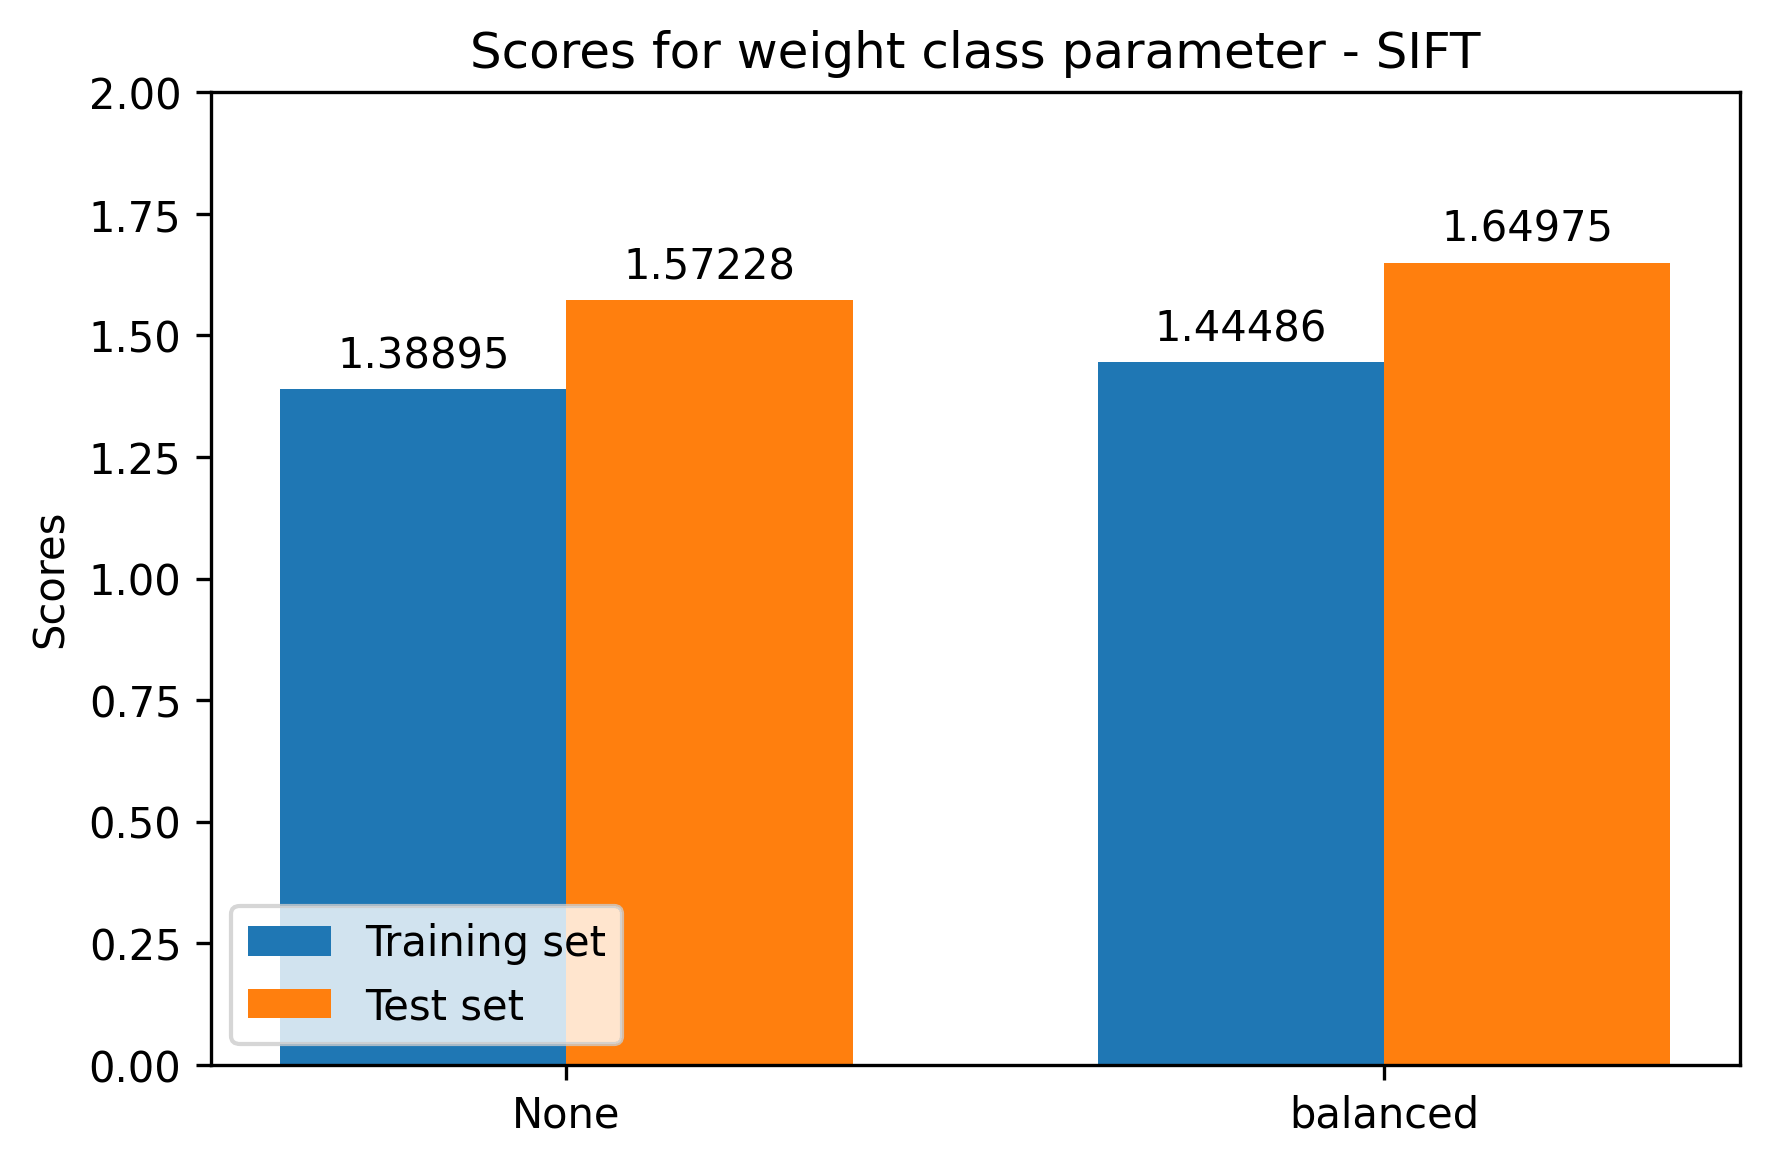
\includegraphics[width=\textwidth]{images/2/2-LBM-model_weight_class.png}}
        \captionsetup{width=0.9\linewidth}
        \captionsetup{justification=centering}
        \caption{Scores for different class\_weight parameters.}
    \end{subfigure}
    \hspace{1cm}
    \begin{subfigure}{.45\textwidth}
        \centering
        \fbox{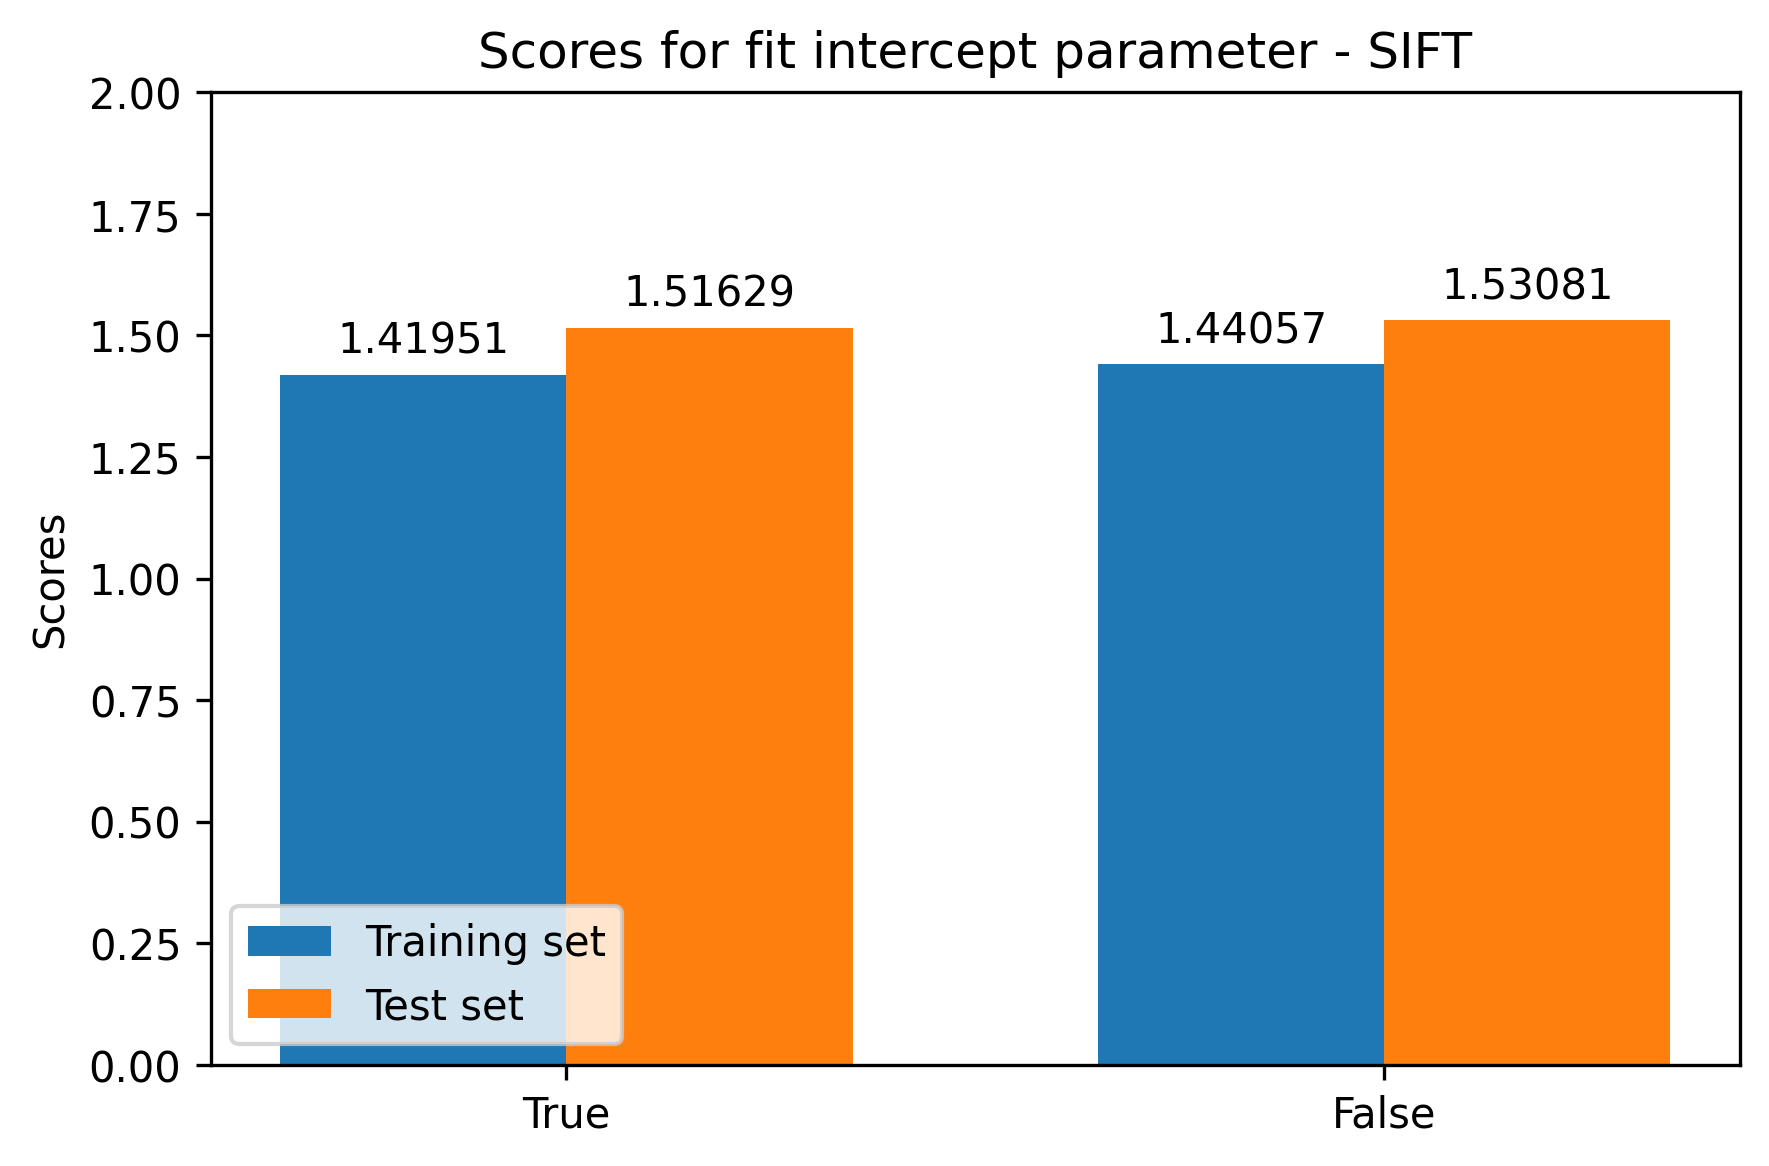
\includegraphics[width=\textwidth]{images/2/2-LBM-model_fit_intercept.png}}
        \captionsetup{width=0.9\linewidth}
        \captionsetup{justification=centering}
        \caption{Scores for different fit\_intercept parameters.}
    \end{subfigure}
    \captionsetup{width=0.8\linewidth}
    \captionsetup{justification=centering}
    \caption{Average multi-class Log Loss score over 10 trials for different model settings.}
    \label{fig:2-weightfit}
\end{figure*}

The default value for the maximum allowed iterations is 100.
With the current settings, convergence is not always reached after 100 iterations.
The following values were tried: 50, 100, 150, 200 and 250.
Since convergence is reached after 250 times in all test cases, this value is used for maximum iterations.


Finally the \textit{hyperparameter} C has to be optimized.
This was done by using \texttt{GridSearchCV} from the Sci Kit Learn library.
This performs an exhaustive search over specified parameter values for the model.
A similar result should be reached by performing the more manual methods used for previous parameters.
In this case the following potential C values were tried: 0.00001, 0.0001, 0.001, 0.01 , 0.1, 0.5, 1.0, 1.5, 3, 5, 10, 100, 1000, 10000
According to Grid Search, 3 is the best value for C, which happens to be close to the default of 1.
If doing the same experiment with the manual method used for the other parameters, the same can be concluded.
This manual method is visualised in figure \ref{fig:2-LBM-model_manual_c}.
This also shows the manual method is most likely just as good and offers greater insight into the working.

\begin{figure}[H]
    \begin{center}
        \fbox{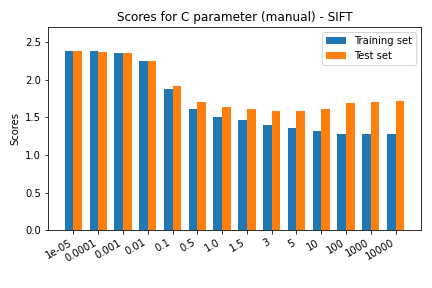
\includegraphics[width=0.75\linewidth]{images/2/2-LBM-model_manual_c.png}}
    \end{center}
    \captionsetup{width=0.6\linewidth}
    \captionsetup{justification=centering}
    \caption{Experimenting with different C values.}
    \label{fig:2-LBM-model_manual_c}
\end{figure}

%------------------------------------

\section{The optimal settings for this model}
\label{section:LBM_optimal}

After all the fine-tuning discussed in the previous sections, an optimal model can be formed.
The optimal settings and received score for the SIFT descriptor are:
\begin{itemize}
    \item Descriptor used: SIFT
    \item Cluster amounts: 100
    \item Sample size: 15\%
    \item Class weight: None
    \item C: 3
    \item Max it-er: 250
    \item Fit intercept: false
    \item Score received from validation set: ± 1.55
    \item Score received on Kaggle: 1.60289
\end{itemize}



